\documentclass[11pt,a4paper]{article}
\usepackage[T1]{fontenc}
\usepackage[utf8]{inputenc}
\usepackage{mathpazo}
\renewcommand{\ttdefault}{pcr}
\usepackage[margin=2.2cm]{geometry}
\usepackage{amsmath,amssymb}
\usepackage{booktabs,array}
\usepackage{enumitem}
\usepackage{xcolor}
\usepackage[most]{tcolorbox}
\usepackage{tikz}\usetikzlibrary{shapes.geometric}
\usepackage{pgfplots}\pgfplotsset{compat=1.18}
\usepackage{fancyhdr}
\usepackage{hyperref}
\hypersetup{colorlinks=true,linkcolor=blue!50!black,urlcolor=blue!50!black}

\definecolor{accent}{RGB}{31,78,121}
\definecolor{solbg}{RGB}{236,246,238}
\definecolor{solfr}{RGB}{46,125,50}

\newif\ifsol
\ifdefined\withsolutions \soltrue \else \solfalse \fi

\newcounter{exo}
\newenvironment{exercise}[1]{\refstepcounter{exo}\par\medskip
  \noindent{\large\bfseries\color{accent} Exercise \theexo\quad #1}\par\smallskip}{\par}
\newtcolorbox{solbox}{colback=solbg,colframe=solfr,boxrule=0.6pt,arc=2pt,
  left=6pt,right=6pt,top=4pt,bottom=4pt,breakable,
  title={\small\bfseries Solution},fonttitle=\color{white},coltitle=white}
\newcommand{\sol}[1]{\ifsol\begin{solbox}#1\end{solbox}\fi}

\pagestyle{fancy}\fancyhf{}
\lhead{\small Practical Machine Learning}
\rhead{\small Sayan CHAKI \textperiodcentered{} LIRIS, Université Lyon 2}
\cfoot{\small\thepage}

\setlist[enumerate,1]{label=\textbf{(\alph*)},leftmargin=*}

\begin{document}

\begin{center}
{\LARGE\bfseries\color{accent} Pen-and-Paper Exercises}\\[4pt]
{\large $k$-Nearest Neighbours, $K$-Means and Linear Regression}\\[4pt]
\ifsol{\large\color{solfr}\bfseries With complete solutions}\else{\normalsize No calculator needed, except where marked with $\bigstar$.}\fi
\end{center}

\noindent\textbf{How to work.} Show every intermediate step: distances, assignments, sums. A correct
number with no working earns no credit in the exam. When a question asks for an interpretation,
answer in two or three sentences and quote your numbers.

\medskip\hrule\medskip

%======================================================================
\section*{Part I \quad $k$-Nearest Neighbours}

\begin{exercise}{Classifying a point by hand}
Seven labelled points in the plane belong to two classes, circles ($\circ$) and triangles ($\triangle$).
We want to classify the query point $q=(3,2)$.

\begin{minipage}{0.48\textwidth}
\centering
\begin{tabular}{cccc}
\toprule
Point & $x_1$ & $x_2$ & Class\\
\midrule
$P_1$ & 1 & 3 & $\circ$\\
$P_2$ & 2 & 2 & $\circ$\\
$P_3$ & 3 & 4 & $\triangle$\\
$P_4$ & 4 & 1 & $\triangle$\\
$P_5$ & 5 & 3 & $\triangle$\\
$P_6$ & 2 & 5 & $\circ$\\
$P_7$ & 6 & 2 & $\circ$\\
\bottomrule
\end{tabular}
\end{minipage}\hfill
\begin{minipage}{0.48\textwidth}
\centering
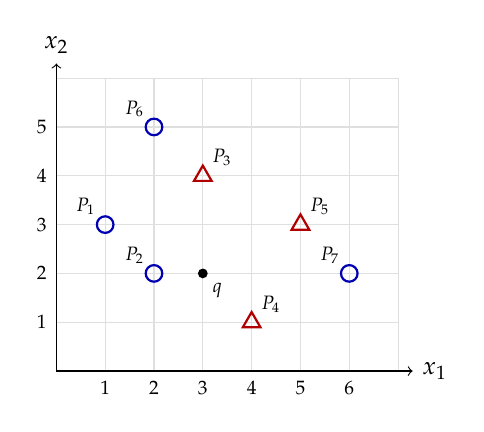
\begin{tikzpicture}[scale=0.62]
\draw[step=1,gray!25] (0,0) grid (7,6);
\draw[->] (0,0)--(7.3,0) node[right]{\small $x_1$};
\draw[->] (0,0)--(0,6.3) node[above]{\small $x_2$};
\foreach \x in {1,...,6} \node[below] at (\x,0) {\scriptsize \x};
\foreach \y in {1,...,5} \node[left] at (0,\y) {\scriptsize \y};
\foreach \p/\l in {{(1,3)}/P_1,{(2,2)}/P_2,{(2,5)}/P_6,{(6,2)}/P_7}
  {\draw[thick,blue!70!black] \p circle (0.17); \node[above left,font=\scriptsize] at \p {$\l$};}
\foreach \p/\l in {{(3,4)}/P_3,{(4,1)}/P_4,{(5,3)}/P_5}
  {\node[regular polygon,regular polygon sides=3,draw=red!70!black,thick,inner sep=1.3pt] at \p {};
   \node[above right,font=\scriptsize] at \p {$\l$};}
\fill[black] (3,2) circle (0.1) node[below right,font=\scriptsize] {$q$};
\end{tikzpicture}
\end{minipage}

\begin{enumerate}
\item Compute the Euclidean distance from $q$ to each $P_i$ (you may keep squared distances for the ranking) and sort the points from nearest to farthest.
\item Predict the class of $q$ with $k=1$, $k=3$, $k=5$ and $k=7$.
\item What does the $k=7$ classifier predict for \emph{any} query point? Explain why a very large $k$ underfits.
\item Repeat the $k=3$ prediction with the Manhattan distance $d_1(u,v)=|u_1-v_1|+|u_2-v_2|$. Does the prediction change?
\item $\bigstar$ In \emph{distance-weighted} $k$-NN, each neighbour votes with weight $1/d(q,P_i)$. Give the prediction for $k=5$ (Euclidean). Compare with (b).
\end{enumerate}

\sol{
\textbf{(a)} Squared distances $d^2=(x_1-3)^2+(x_2-2)^2$:\\[3pt]
\centerline{\begin{tabular}{lccccccc}
\toprule
& $P_2$ & $P_4$ & $P_3$ & $P_1$ & $P_5$ & $P_7$ & $P_6$\\
\midrule
$d^2$ & 1 & 2 & 4 & 5 & 5 & 9 & 10\\
$d$ & 1 & 1.414 & 2 & 2.236 & 2.236 & 3 & 3.162\\
class & $\circ$ & $\triangle$ & $\triangle$ & $\circ$ & $\triangle$ & $\circ$ & $\circ$\\
$d_1$ & 1 & 2 & 2 & 3 & 3 & 3 & 4\\
\bottomrule
\end{tabular}}\\[3pt]
\textbf{(b)} $k=1$: $\{P_2\}$ gives $\circ$.\quad $k=3$: $\{P_2,P_4,P_3\}$ gives 2 $\triangle$ vs 1 $\circ$, so $\triangle$.\quad
$k=5$: adds $P_1(\circ)$ and $P_5(\triangle)$: 3 $\triangle$ vs 2 $\circ$, so $\triangle$.\quad
$k=7$: all points, 4 $\circ$ vs 3 $\triangle$, so $\circ$. The prediction flips twice as $k$ grows.

\textbf{(c)} With $k=n=7$ every query has the same neighbourhood (the whole training set), so the classifier always predicts the majority class $\circ$. It ignores the position of $q$ entirely: this is maximal bias, the extreme case of underfitting.

\textbf{(d)} Manhattan distances are in the last row. The three nearest are $P_2$ (1), then $P_4$ and $P_3$ (both 2; the fourth nearest is at distance 3, so there is no ambiguity about who enters). The vote is again $\triangle$. The ranking changed (here $P_3$ and $P_4$ are tied) but the prediction did not.

\textbf{(e)} Weights $1/d$: $\circ$ gets $1/1+1/\sqrt5\approx 1+0.447=1.447$;
$\triangle$ gets $1/\sqrt2+1/2+1/\sqrt5\approx 0.707+0.5+0.447=1.654$. Prediction $\triangle$, as in (b), but the margin is much smaller (1.654 vs 1.447 instead of 3 votes vs 2) because the single closest point $P_2$ now weighs as much as two farther points.
}
\end{exercise}

\begin{exercise}{Choosing $k$ by leave-one-out}
A one-dimensional training set with two classes $A$ and $B$:
\[
\begin{array}{c|cccccccc}
x & 1 & 2 & 4 & 5 & 8 & 9 & 11 & 15\\\hline
\text{class} & A & A & A & B & B & A & B & B
\end{array}
\]
In \emph{leave-one-out} (LOO) validation, each point in turn is removed, classified by $k$-NN using the 7 remaining points, and compared with its true label.
\begin{enumerate}
\item Compute the LOO error (number of mistakes out of 8) for $k=1$. Present your work as a table: point, neighbour(s), prediction, correct or not.
\item Same for $k=3$ and $k=5$.
\item Which $k$ would you choose? Point to the specific training points that make $k=1$ perform badly and explain what they represent.
\item Why is it forbidden to include the point itself among its neighbours when computing this error? What would the error of 1-NN be if we did?
\end{enumerate}

\sol{
\textbf{(a) $k=1$.}\\[2pt]
\centerline{\begin{tabular}{cccccccccc}
\toprule
$x$ & 1 & 2 & 4 & 5 & 8 & 9 & 11 & 15\\
true & $A$ & $A$ & $A$ & $B$ & $B$ & $A$ & $B$ & $B$\\
nearest & 2 & 1 & 5 & 4 & 9 & 8 & 9 & 11\\
predicted & $A$ & $A$ & $B$ & $A$ & $A$ & $B$ & $A$ & $B$\\
& \checkmark & \checkmark & $\times$ & $\times$ & $\times$ & $\times$ & $\times$ & \checkmark\\
\bottomrule
\end{tabular}}
LOO error $=5/8$.

\textbf{(b) $k=3$.} Neighbours (by increasing distance) and votes:
$1\!:\{2,4,5\}=AAB\to A$ \checkmark;\;
$2\!:\{1,4,5\}=AAB\to A$ \checkmark;\;
$4\!:\{5,2,1\}=BAA\to A$ \checkmark;\;
$5\!:\{4,2,8\}=AAB\to A$ $\times$;\;
$8\!:\{9,5,11\}=ABB\to B$ \checkmark;\;
$9\!:\{8,11,5\}=BBB\to B$ $\times$;\;
$11\!:\{9,8,15\}=ABB\to B$ \checkmark;\;
$15\!:\{11,9,8\}=BAB\to B$ \checkmark.
LOO error $=2/8$.

\textbf{$k=5$.}
$1\!:AABBA\to A$ \checkmark;\; $2\!:AABBA\to A$ \checkmark;\; $4\!:BAABA\to A$ \checkmark;\;
$5\!:AABAA\to A$ $\times$;\; $8\!:\{9,5,11,4,2\}=ABBAA\to A$ $\times$;\; $9\!:BBBAB\to B$ $\times$;\;
$11\!:ABBBA\to B$ \checkmark;\; $15\!:BABBA\to B$ \checkmark.
LOO error $=3/8$. (For $x=8$, points 5 and 11 are both at distance 3; both are among the 5 nearest, so the tie does not matter.)

\textbf{(c)} Choose $k=3$ (error $2/8$). The point $x=9$ labelled $A$ sits inside a run of $B$'s and $x=5$ labelled $B$ sits next to $A$'s: they behave like label noise. With $k=1$ each of them corrupts the prediction of its neighbours (4, 8, 11 are all misclassified because of them). $k=3$ averages them out; $k=5$ starts to blur the true boundary between the two classes around $x\approx 6$.

\textbf{(d)} A point is always at distance 0 from itself, so 1-NN would predict its own label and the error would be $0/8$ for any data set. The estimate would measure memorisation, not generalisation. LOO is a special case of cross-validation with $n$ folds.
}
\end{exercise}

\begin{exercise}{Why features must be scaled}
A bank describes customers by age (years) and annual income (euros). Query customer $q=(30,\ 40\,000)$. Two stored customers:
$a=(32,\ 52\,000)$ and $b=(55,\ 41\,000)$.
\begin{enumerate}
\item Compute $d(q,a)$ and $d(q,b)$ in raw units. Which customer is nearer? Which feature decides?
\item On the training set, age has standard deviation 10 years and income has standard deviation $10\,000$ euros. Standardise the \emph{differences} (divide each difference by its feature's standard deviation) and recompute both distances. Which customer is nearer now?
\item Would expressing income in thousands of euros instead of euros change the answer to (a)? What does this tell you about unscaled $k$-NN?
\item The standard deviations must be computed on the training set only. Explain why, and name the scikit-learn object that makes this automatic.
\end{enumerate}

\sol{
\textbf{(a)} $d(q,a)=\sqrt{2^2+12\,000^2}\approx 12\,000.0$ and $d(q,b)=\sqrt{25^2+1\,000^2}\approx 1\,000.3$. So $b$ is nearer. Income decides alone: an age gap of 25 years adds only 0.3 to the distance.

\textbf{(b)} For $a$: $(2/10,\ 12\,000/10\,000)=(0.2,\ 1.2)$, $d=\sqrt{0.04+1.44}\approx 1.217$.
For $b$: $(25/10,\ 1\,000/10\,000)=(2.5,\ 0.1)$, $d=\sqrt{6.25+0.01}\approx 2.502$. Now $a$ is nearer.

\textbf{(c)} Yes. In thousands of euros, $d(q,a)=\sqrt{4+144}\approx 12.2$ and $d(q,b)=\sqrt{625+1}\approx 25.0$, so $a$ becomes nearer. The neighbours of a point depend on the arbitrary choice of units: unscaled $k$-NN is not a well-defined method until the scales are fixed.

\textbf{(d)} Using test data to compute the scaling leaks information about the test set into the model, and the test score is then optimistic. A \texttt{Pipeline} (e.g.\ \texttt{make\_pipeline(StandardScaler(), KNeighborsClassifier())}) fits the scaler on the training folds only, including inside cross-validation.
}
\end{exercise}

\begin{exercise}{The curse of dimensionality \quad$\bigstar$}
Data points are spread uniformly in the unit hypercube $[0,1]^d$. We want a small sub-cube around a query point that contains a fraction $p$ of the data, i.e.\ a sub-cube of volume $p$.
\begin{enumerate}
\item Show that the side length of this sub-cube is $e_d(p)=p^{1/d}$.
\item Compute $e_d(0.01)$ for $d=1,2,10,100$.
\item Interpret: are the ``$1\%$ nearest neighbours'' in dimension 100 still \emph{near}? What does this imply for $k$-NN on raw high-dimensional data?
\end{enumerate}

\sol{
\textbf{(a)} A cube of side $e$ in dimension $d$ has volume $e^d$. Setting $e^d=p$ gives $e=p^{1/d}$.

\textbf{(b)} $e_1=0.01$, $e_2=0.1$, $e_{10}=0.01^{0.1}\approx 0.63$, $e_{100}=0.01^{0.01}\approx 0.955$.

\textbf{(c)} In dimension 100, capturing only $1\%$ of the data requires covering $95.5\%$ of the range of \emph{every} feature. The ``neighbourhood'' is almost the whole space, so the neighbours are not similar to the query and the local-averaging idea behind $k$-NN breaks down. Remedies: feature selection, dimensionality reduction (e.g.\ PCA), or a model that does not rely on local neighbourhoods.
}
\end{exercise}

%======================================================================
\section*{Part II \quad $K$-Means}

Recall the two steps of Lloyd's algorithm: \emph{assign} each point to its nearest centre, then \emph{update} each centre to the mean of its points. The \emph{inertia} is $J=\sum_i \lVert x_i-\mu_{c(i)}\rVert^2$.

\begin{exercise}{Running $K$-means by hand; the role of initialisation}
One-dimensional data: $\quad 1,\ 2,\ 3,\ 8,\ 9,\ 10,\ 25.\quad$ We use $K=2$.
\begin{enumerate}
\item \textbf{Initialisation A:} $\mu_1=1$, $\mu_2=2$. Run Lloyd's algorithm until the assignments stop changing. At each iteration, write the decision threshold $(\mu_1+\mu_2)/2$, the two clusters and the new centres.
\item Compute the final inertia for initialisation A.
\item \textbf{Initialisation B:} $\mu_1=1$, $\mu_2=25$. Run the algorithm to convergence and compute the final inertia.
\item Both runs have converged, yet the inertias differ. What does this tell you about Lloyd's algorithm? How does scikit-learn's \texttt{n\_init} parameter address it?
\item Compute the inertia of the partition $\{1,2,3\},\{8,9,10\},\{25\}$ ($K=3$). Given your results, discuss whether $25$ is best seen as a cluster or as an outlier.
\end{enumerate}

\sol{
\textbf{(a) Initialisation A.}\\
Iter.~1: threshold $1.5$. Clusters $\{1\}$ and $\{2,3,8,9,10,25\}$. Centres $\mu_1=1$, $\mu_2=57/6=9.5$.\\
Iter.~2: threshold $(1+9.5)/2=5.25$. Clusters $\{1,2,3\}$ and $\{8,9,10,25\}$. Centres $\mu_1=2$, $\mu_2=52/4=13$.\\
Iter.~3: threshold $7.5$. Same clusters: converged.

\textbf{(b)} $J_A=(1+0+1)+(25+16+9+144)=2+194=196$.

\textbf{(c) Initialisation B.} Iter.~1: threshold $13$. Clusters $\{1,2,3,8,9,10\}$ and $\{25\}$. Centres $\mu_1=33/6=5.5$, $\mu_2=25$.
Iter.~2: threshold $15.25$: same clusters, converged.
$J_B=(4.5^2+3.5^2+2.5^2+2.5^2+3.5^2+4.5^2)+0=20.25+12.25+6.25+6.25+12.25+20.25=77.5$.

\textbf{(d)} Lloyd's algorithm only guarantees convergence to a \emph{local} minimum of $J$ (a partition that neither step can improve). A bad start (two centres inside the same group) gets trapped at $J=196$, while $J=77.5$ is the global optimum here. \texttt{n\_init} runs the algorithm from several initialisations and keeps the run with the lowest inertia.

\textbf{(e)} $J=(1+0+1)+(1+0+1)+0=4$. Going from $K=2$ to $K=3$ divides the inertia by almost 20, a very strong elbow at $K=3$. Note that the best $K=2$ solution isolates 25 on its own: because $J$ uses \emph{squared} distances, a single far point pulls a whole centre towards it. Whether 25 is a genuine cluster of size one or a measurement error cannot be decided by $K$-means; it must be checked against domain knowledge.
}
\end{exercise}

\begin{exercise}{$k$-means++ initialisation}
With the same data $1,2,3,8,9,10,25$, $k$-means++ picks the first centre uniformly at random; suppose it picks $1$. Each next centre is drawn with probability proportional to $D(x)^2$, the squared distance from $x$ to the nearest centre already chosen.
\begin{enumerate}
\item Compute $D(x)^2$ for every point and the probability of each being picked as the second centre.
\item What is the probability that the second centre is 25? Is this good or bad news for these data, given Exercise 5?
\item Explain in one sentence why $k$-means++ is sensitive to outliers.
\end{enumerate}

\sol{
\textbf{(a)} $D^2$: $0,1,4,49,64,81,576$; total $775$. Probabilities for $x=1,2,3,8,9,10,25$:
\[ 0,\ \tfrac{1}{775},\ \tfrac{4}{775},\ \tfrac{49}{775},\ \tfrac{64}{775},\ \tfrac{81}{775},\ \tfrac{576}{775}\ \approx\ 0,\ 0.001,\ 0.005,\ 0.063,\ 0.083,\ 0.105,\ 0.743. \]

\textbf{(b)} $P(25)=576/775\approx 0.74$. For $K=2$ this is good news: starting from $\{1,25\}$ is exactly initialisation B, which leads to the global optimum $J=77.5$. The other likely choices (8, 9, 10) also end at $J=77.5$ or close; picking 2 or 3 (probability about $0.6\%$) risks the bad optimum.

\textbf{(c)} Squared distances make isolated far points very likely to be chosen as centres, so an outlier tends to receive a centre of its own.
}
\end{exercise}

\begin{exercise}{Why Lloyd's algorithm never increases the inertia}
\begin{enumerate}
\item Let $x_1,\dots,x_m\in\mathbb R^p$ be the points of one cluster. Show that $f(\mu)=\sum_{j=1}^m\lVert x_j-\mu\rVert^2$ is minimised at $\mu=\bar x=\frac1m\sum_j x_j$. (Compute the gradient.)
\item Explain why the \emph{assignment} step cannot increase $J$, and why the \emph{update} step cannot increase $J$.
\item Deduce that the algorithm stops after a finite number of iterations. (Hint: how many partitions of $n$ points into $K$ groups exist?)
\end{enumerate}

\sol{
\textbf{(a)} $\nabla f(\mu)=-2\sum_j (x_j-\mu)=-2\big(\sum_j x_j - m\mu\big)$. Setting it to zero gives $\mu=\bar x$. The Hessian is $2m\,I$, positive definite, so $f$ is strictly convex and $\bar x$ is its unique minimiser.

\textbf{(b)} Assignment: with centres fixed, each term $\lVert x_i-\mu_{c(i)}\rVert^2$ is replaced by the smallest possible value $\min_k \lVert x_i-\mu_k\rVert^2$, so no term increases. Update: with assignments fixed, $J$ is a sum of independent functions of the form in (a), one per cluster, and each is replaced by its minimum. Hence $J$ is non-increasing across iterations.

\textbf{(c)} There are finitely many partitions (at most $K^n$). $J$ is determined by the partition once centres are updated, and it strictly decreases whenever the partition changes (with a consistent tie-breaking rule), so no partition can be visited twice. The algorithm must therefore stop after finitely many iterations, at a local minimum.
}
\end{exercise}

%======================================================================
\section*{Part III \quad Linear Regression}

Throughout this part we use the five observations
\[
\begin{array}{c|ccccc}
x & 1 & 2 & 3 & 4 & 5\\\hline
y & 2 & 3 & 5 & 4 & 6
\end{array}
\]
and the model $\hat y = wx+b$ fitted by minimising the mean squared error $L(w,b)=\frac1n\sum_i (y_i-wx_i-b)^2$.

\begin{exercise}{The least-squares line by hand}
\begin{enumerate}
\item Derive the closed-form solution by setting $\partial L/\partial b=0$ and $\partial L/\partial w=0$. Show that
\[ b=\bar y-w\bar x,\qquad w=\frac{S_{xy}}{S_{xx}},\quad S_{xy}=\sum_i(x_i-\bar x)(y_i-\bar y),\ S_{xx}=\sum_i(x_i-\bar x)^2. \]
\item Compute $\bar x,\bar y,S_{xx},S_{xy}$, then $w$ and $b$.
\item Compute the fitted values, the residuals $e_i=y_i-\hat y_i$, and check that $\sum_i e_i=0$. Explain why this always holds when the model has an intercept.
\item Compute $SSE=\sum e_i^2$, $SST=\sum (y_i-\bar y)^2$ and $R^2=1-SSE/SST$. Interpret $R^2$ in one sentence.
\item Predict $y$ at $x=6$. Would you trust a prediction at $x=50$? Why?
\end{enumerate}

\sol{
\textbf{(a)} $\partial L/\partial b=-\frac2n\sum(y_i-wx_i-b)=0\Rightarrow b=\bar y-w\bar x$. Substituting,
$\partial L/\partial w=-\frac2n\sum x_i\big((y_i-\bar y)-w(x_i-\bar x)\big)=0$. Since $\sum \bar x\,(y_i-\bar y)=0$ and $\sum\bar x\,(x_i-\bar x)=0$, we may replace $x_i$ by $x_i-\bar x$: $\sum (x_i-\bar x)(y_i-\bar y)=w\sum(x_i-\bar x)^2$, so $w=S_{xy}/S_{xx}$.

\textbf{(b)} $\bar x=3$, $\bar y=20/5=4$. Deviations: $x-\bar x=(-2,-1,0,1,2)$, $y-\bar y=(-2,-1,1,0,2)$.
$S_{xx}=4+1+0+1+4=10$, $S_{xy}=4+1+0+0+4=9$. So $w=0.9$ and $b=4-0.9\times 3=1.3$.

\textbf{(c)} $\hat y=(2.2,\ 3.1,\ 4.0,\ 4.9,\ 5.8)$, $e=(-0.2,\ -0.1,\ 1.0,\ -0.9,\ 0.2)$, and $\sum e_i=0$. This is exactly the equation $\partial L/\partial b=0$: at the optimum, the residuals sum to zero whenever the intercept is free.

\textbf{(d)} $SSE=0.04+0.01+1+0.81+0.04=1.90$; $SST=4+1+1+0+4=10$; $R^2=1-0.19=0.81$. The line explains $81\%$ of the variance of $y$ around its mean.

\textbf{(e)} $\hat y(6)=0.9\times 6+1.3=6.7$. At $x=50$ the model gives $46.3$, but this is extrapolation far outside the observed range $[1,5]$: nothing in the data supports the assumption that the relationship stays linear there.
}
\end{exercise}

\begin{exercise}{The normal equations}
Write the model as $\hat{\mathbf y}=X\boldsymbol\theta$ with $\boldsymbol\theta=(b,w)^\top$ and a design matrix $X$ whose first column is all ones.
\begin{enumerate}
\item Write $X$ and compute $X^\top X$ and $X^\top \mathbf y$.
\item Solve $X^\top X\,\boldsymbol\theta=X^\top\mathbf y$ by inverting the $2\times 2$ matrix. Check that you recover Exercise 8.
\item Suppose we add a third column equal to $2x$. What happens to $X^\top X$? What does this mean for the solution, and how does Ridge regression fix it?
\end{enumerate}

\sol{
\textbf{(a)} $X=\begin{pmatrix}1&1&1&1&1\\1&2&3&4&5\end{pmatrix}^{\!\top}$,\quad
$X^\top X=\begin{pmatrix}5&15\\15&55\end{pmatrix}$,\quad
$X^\top\mathbf y=\begin{pmatrix}\sum y_i\\ \sum x_iy_i\end{pmatrix}=\begin{pmatrix}20\\69\end{pmatrix}$ \ (since $2+6+15+16+30=69$).

\textbf{(b)} $\det=5\cdot55-15^2=50$, $(X^\top X)^{-1}=\frac1{50}\begin{pmatrix}55&-15\\-15&5\end{pmatrix}$.
$b=\frac{55\cdot20-15\cdot69}{50}=\frac{65}{50}=1.3$, \ $w=\frac{-15\cdot20+5\cdot69}{50}=\frac{45}{50}=0.9$. Same as before.

\textbf{(c)} The third column is a linear combination of the second, so $X$ has rank 2, $X^\top X$ is $3\times3$ but singular ($\det=0$) and has no inverse. Infinitely many $\boldsymbol\theta$ give the same fit (any split of the slope between $x$ and $2x$), so the coefficients are not identifiable. Ridge solves $(X^\top X+\lambda I)\boldsymbol\theta=X^\top\mathbf y$; for $\lambda>0$ the matrix is positive definite, hence invertible, and the solution is unique.
}
\end{exercise}

\begin{exercise}{One step of gradient descent}
\begin{enumerate}
\item Show that $\dfrac{\partial L}{\partial w}=-\dfrac2n\sum_i x_i(y_i-\hat y_i)$ and $\dfrac{\partial L}{\partial b}=-\dfrac2n\sum_i (y_i-\hat y_i)$.
\item Start from $w=0,\ b=0$. Compute $L(0,0)$ and both partial derivatives. (Use $\sum x_iy_i=69$, $\sum y_i=20$, $\sum y_i^2=90$.)
\item Perform one update with learning rate $\eta=0.05$: $\ w\leftarrow w-\eta\,\partial L/\partial w$, $\ b\leftarrow b-\eta\,\partial L/\partial b$.
\item $\bigstar$ Compute $L$ after the step. Did the loss decrease? Compare the new $(w,b)$ with the optimum $(0.9,1.3)$: which parameter overshot, and why is that not a contradiction?
\end{enumerate}

\sol{
\textbf{(a)} Chain rule on $(y_i-wx_i-b)^2$: derivative w.r.t.\ $w$ is $2(y_i-\hat y_i)(-x_i)$, w.r.t.\ $b$ is $2(y_i-\hat y_i)(-1)$; average over $i$.

\textbf{(b)} At $(0,0)$, $\hat y=0$: $L=\frac{90}{5}=18$, $\ \partial L/\partial w=-\frac25\cdot 69=-27.6$, $\ \partial L/\partial b=-\frac25\cdot20=-8$.

\textbf{(c)} $w=0+0.05\times27.6=1.38$, $\ b=0+0.05\times 8=0.40$.

\textbf{(d)} $\hat y=(1.78,3.16,4.54,5.92,7.30)$, residuals $(0.22,-0.16,0.46,-1.92,-1.30)$,
$L=\frac{0.0484+0.0256+0.2116+3.6864+1.69}{5}=\frac{5.662}{5}\approx1.13$. The loss dropped from 18 to 1.13. The slope overshot ($1.38>0.9$) while the intercept is still too small ($0.40<1.3$). The gradient points in the steepest direction of $L$ at the current point, not towards the optimum; because $x$ is not centred, $w$ and $b$ are coupled and later steps will trade slope for intercept. Centring $x$ would decouple them and speed up convergence.
}
\end{exercise}

\begin{exercise}{Ridge regression in one dimension}
Centre the data ($\tilde x_i=x_i-\bar x$, $\tilde y_i=y_i-\bar y$) and fit $\tilde y=w\tilde x$ by minimising $\sum_i(\tilde y_i-w\tilde x_i)^2+\lambda w^2$.
\begin{enumerate}
\item Show that $w_\lambda=\dfrac{S_{xy}}{S_{xx}+\lambda}$.
\item Compute $w_\lambda$ for $\lambda=0,\ 5,\ 10,\ 90$ and the intercept $b_\lambda=\bar y-w_\lambda\bar x$ for $\lambda=5$.
\item What happens as $\lambda\to\infty$? Why is the intercept usually \emph{not} penalised?
\item Why must features be standardised before applying Ridge with several features?
\end{enumerate}

\sol{
\textbf{(a)} Derivative: $-2\sum\tilde x_i(\tilde y_i-w\tilde x_i)+2\lambda w=0\Rightarrow w\big(\sum\tilde x_i^2+\lambda\big)=\sum\tilde x_i\tilde y_i$, i.e.\ $w_\lambda=S_{xy}/(S_{xx}+\lambda)$.

\textbf{(b)} $w_0=9/10=0.9$,\ $w_5=9/15=0.6$,\ $w_{10}=9/20=0.45$,\ $w_{90}=9/100=0.09$. For $\lambda=5$: $b_5=4-0.6\times3=2.2$.

\textbf{(c)} $w_\lambda\to0$: the model tends to the constant prediction $\bar y$. Penalising the intercept would pull predictions towards 0, which depends on the arbitrary origin of $y$ (e.g.\ temperatures in Celsius vs Kelvin); shrinking the \emph{slopes} towards 0 means ``the feature has no effect'', which is the intended prior.

\textbf{(d)} The penalty $\lambda\sum_j w_j^2$ treats all coefficients equally, but a coefficient's size depends on its feature's unit (a feature in metres has a coefficient 1000 times larger than the same feature in millimetres). Without standardisation, Ridge would shrink features according to their units rather than their usefulness.
}
\end{exercise}

\begin{exercise}{Outliers and leverage}
Add one observation to the five points and refit by least squares.
\begin{enumerate}
\item Case 1: add $(x,y)=(3,14)$. Compute the new $\bar x,\bar y,S_{xx},S_{xy}$, then $w$ and $b$.
\item Case 2: instead add $(x,y)=(9,4)$. Same computation.
\item Both new points lie far from the original line. Compare the effect on the slope and explain the difference using the notion of \emph{leverage} (distance of $x_i$ from $\bar x$).
\item Name one loss function that is less sensitive to such points than the squared error.
\end{enumerate}

\sol{
\textbf{(a)} $\bar x=18/6=3$, $\bar y=34/6\approx5.667$. The new point has $x-\bar x=0$, so it adds nothing to $S_{xx}=10$ or to $S_{xy}=\sum(x_i-\bar x)y_i=9$ (using $\sum(x_i-\bar x)=0$). Thus $w=0.9$ unchanged, $b=5.667-2.7\approx2.967$: the line just moves up.

\textbf{(b)} $\bar x=24/6=4$, $\bar y=24/6=4$. Deviations $x-\bar x=(-3,-2,-1,0,1,5)$, $y-\bar y=(-2,-1,1,0,2,0)$. $S_{xx}=9+4+1+0+1+25=40$, $S_{xy}=6+2-1+0+2+0=9$. So $w=9/40=0.225$ and $b=4-0.225\times4=3.1$.

\textbf{(c)} The vertical outlier at $x=\bar x$ has zero leverage: it shifts the intercept but cannot tilt the line. The point at $x=9$ is far from the other $x$'s (high leverage) and cuts the slope by a factor of 4, from 0.9 to 0.225, although its $y$ value is perfectly ordinary. Always inspect points with extreme $x$ values.

\textbf{(d)} The absolute loss $|e|$ (least absolute deviations) or the Huber loss, which is quadratic for small residuals and linear for large ones (\texttt{HuberRegressor} in scikit-learn).
}
\end{exercise}

\end{document}
